\documentclass[addpoints,spanish, 12pt,a4paper,cancelspace]{./include/gexam}

 %%%%%%%%%%%%%%%%%%%%%%%%%%%
 \renewcommand{\documentName} { 3ª evaluación }
 \renewcommand{\documentContent} { Sistema de coordenadas cartesianos } 
 \renewcommand{\waterMark} { Modelo 3 } 

 % Configuración del documento.
 \renewcommand{\schoolSubject} { Examen Matemáticas 2º ESO  }
\renewcommand{\school} { IES José de Churriguera  }
\renewcommand{\academicPeriod} { Curso 2022/2023 }

\renewcommand{\autor} { Andrés Giménez Muñoz }
\renewcommand{\emailAuthor} { andresprofemates@outlook.es }
\renewcommand{\autorSing}{ Profesor: Andrés } 
 %%%%%%%%%%%%%%%%%%%%%%%%%%%
 
% \renewcommand{\thepartno}{\arabic{partno}}
%  \renewcommand{\thepartno}{\thecurrentpartno.\arabic{partno}}

% \renewcommand{\partlabel}{$(\thequestion.\arabic{partno})$}
% \renewcommand{\subpartlabel}{$(\thepart.\arabic{subpartno})$}

\renewcommand\subpartlabel{$(\thesubpart)$}
\renewcommand\subpartshook{\renewcommand\makelabel[1]{##1\hfil }} 
 
 %%%%%%%%%%%%%%%%%%%%%%%%%%%
 % Exam configuration
 %\pointsdroppedatright   %% No mostrar la puntuación
 \pointsinrightmargin{} % Para poner las puntuaciones a la derecha. Se puede cambiar. Si se comenta, sale a la izquierda.
 \extrawidth{-1.5cm} %Un poquito más de margen por si ponemos textos largos.
 \marginpointname{ \emph{\points}}
 
 %% Si se comenta no aparecerán los espacios de la solución.
 %\nocancelspace
 
 %% Puntuación a la izquierda.
%  \nopointsinrightmargin 

 %% Esto es de la clase exam. Si dejamos sin comentar \printanswers, se mostraran las soluciones. 
 %% Si la comentamos y dejamos sin comentar \noprintanswers, pues no se muestran las soluciones.
 % \printanswers
 %\noprintanswers
 
 %%%%%%%%%%%%%%%%%%%%%%%%%%%
 
 \begin{document}
 
%  \StudentData{}
%  \GradeTableHeader{}
 
 \justifying

% \begin{center}
%     \fbox{\fbox{\parbox{6.5in}{             
%                 \begin{itemize}
%                     \item Deben aparecer todas las operaciones, no vale solo con indicar el resultado.
%                     \item Se podrán quitar hasta cinco décimas por falta de claridad o rigor en el desarrollo de las respuestas o por una mala presentación.
%                     \item Se valorará que se indiquen las cuentas en línea, realizando las operaciones en el margen.
%                     \item No se puede utilizar la calculadora.
%                 \end{itemize}
%             }}}
% \end{center}
 
 \begin{questions}
    
    %% Gato
    \question Dibuja los puntos en el orden en el que aparece y únelos con segmentos de línea. \\
    Trazo 1 [Negro]:
    \\
    $(0,26)$, $(3,27)$, $(7,28)$, $(15,29)$, $(20,28)$, $(25,27)$, $(31,25)$, $(35,23)$, $(36,23)$, $(37,24)$, $(38,28)$, $(38,37)$, $(45,30)$, $(56,30)$, $(60,33)$,
    $(62,34)$, $(64,35)$, $(63,25)$, $(62,21)$, $(63,16)$, $(61,13)$, $(56,8)$, $(54,5)$, $(50,-4)$, $(39,-21)$, $(35,-40)$, $(36,-45)$, $(37,-46)$, $(39,-47)$, $(40,-48)$, $(40,-50)$,
    $(32,-50)$, $(31,-48)$, $(30,-40)$, $(29,-30)$, $(27,-24)$, $(27,-30)$, $(26,-44)$, $(25,-46)$, $(23,-48)$, $(21,-48)$, $(19,-45)$, $(19,-40)$, $(20,-35)$, $(20,-30)$, $(18,-25)$,
    $(15,-19)$, $(12,-15)$, $(10,-16)$, $(7,-20)$, $(-5,-34)$, $(1,-41)$
    \\
    Trazo 2 [Negro]:
    \\
    $(1,-41)$, $(2,-42)$, $(5,-42)$, $(7,-44)$, $(6,-46)$, $(-1,-46)$, $(-16,-32)$, $(-19,-36)$, $(-14,-44)$, $(-11,-45)$, $(-10,-46)$, $(-10,-48)$, $(-11,-49)$,
    $(-17,-49)$, $(-18,-48)$, $(-27,-32)$, $(-27,-30)$, $(-25,-22)$, $(-27,-15)$, $(-29,-9)$, $(-32,-4)$, $(-35,-4)$, $(-40,-3)$, $(-46,0)$, $(-50,3)$, $(-54,8)$, $(-56,14)$, $(-56,18)$,
    $(-55,22)$, $(-53,26)$, $(-50,30)$, $(-46,33)$, $(-40,37)$, $(-37,38)$, $(-34,38)$, $(-33,37)$, $(-37,35)$, $(-46,27)$, $(-49,21)$, $(-50,19)$, $(-50,15)$, $(-47,10)$, $(-43,6)$, $(-36,3)$,
    $(-33,3)$, $(-30,6)$, $(-26,10)$, $(-21,15)$, $(-15,20)$, $(-9,23)$, $(-4,25)$, $(0,26)$
    \\
    Trazo 3 [Rojo con relleno naranja]:
    \\
    $(53,17)$, $(54,18)$, $(56,19)$, $(60,18)$, $(57,16)$, $(54,16)$, $(53,17)$
    \\
    Trazo 4 [Rojo con relleno naranja]:
    \\
    $(42,20)$, $(47,19)$, $(48,18)$, $(47,16)$, $(45,16)$, $(43,18)$, $(42,20)$
    \\

    % \begin{tikzpicture}[scale=1]
    %     \begin{axis}[
    %         axis x line=center,
    %         axis y line=center,
    %         xmin=-60,xmax=60,
    %         ymin=-60,ymax=60,
    %         grid=both,
    %         grid style={line width=.1pt, draw=gray!10},
    %         major grid style={line width=.2pt,draw=gray!50},
    %         axis lines=middle,
    %         axis line style={<->},
    %         minor tick num=4,
    %         enlargelimits={abs=0.5},
    %         axis line style={latex-latex},
    %         % ticklabel style={font=\tiny,fill=white},
    %         % xlabel style={at={$(ticklabel* cs:1)$},anchor=north west},
    %         % ylabel style={at={$(ticklabel* cs:1)$},anchor=south west},
    %         xlabel style={below right},
    %         ylabel style={above left},
    %         width=17cm,
    %     ]
        
    %     \end{axis}

    % \end{tikzpicture}

    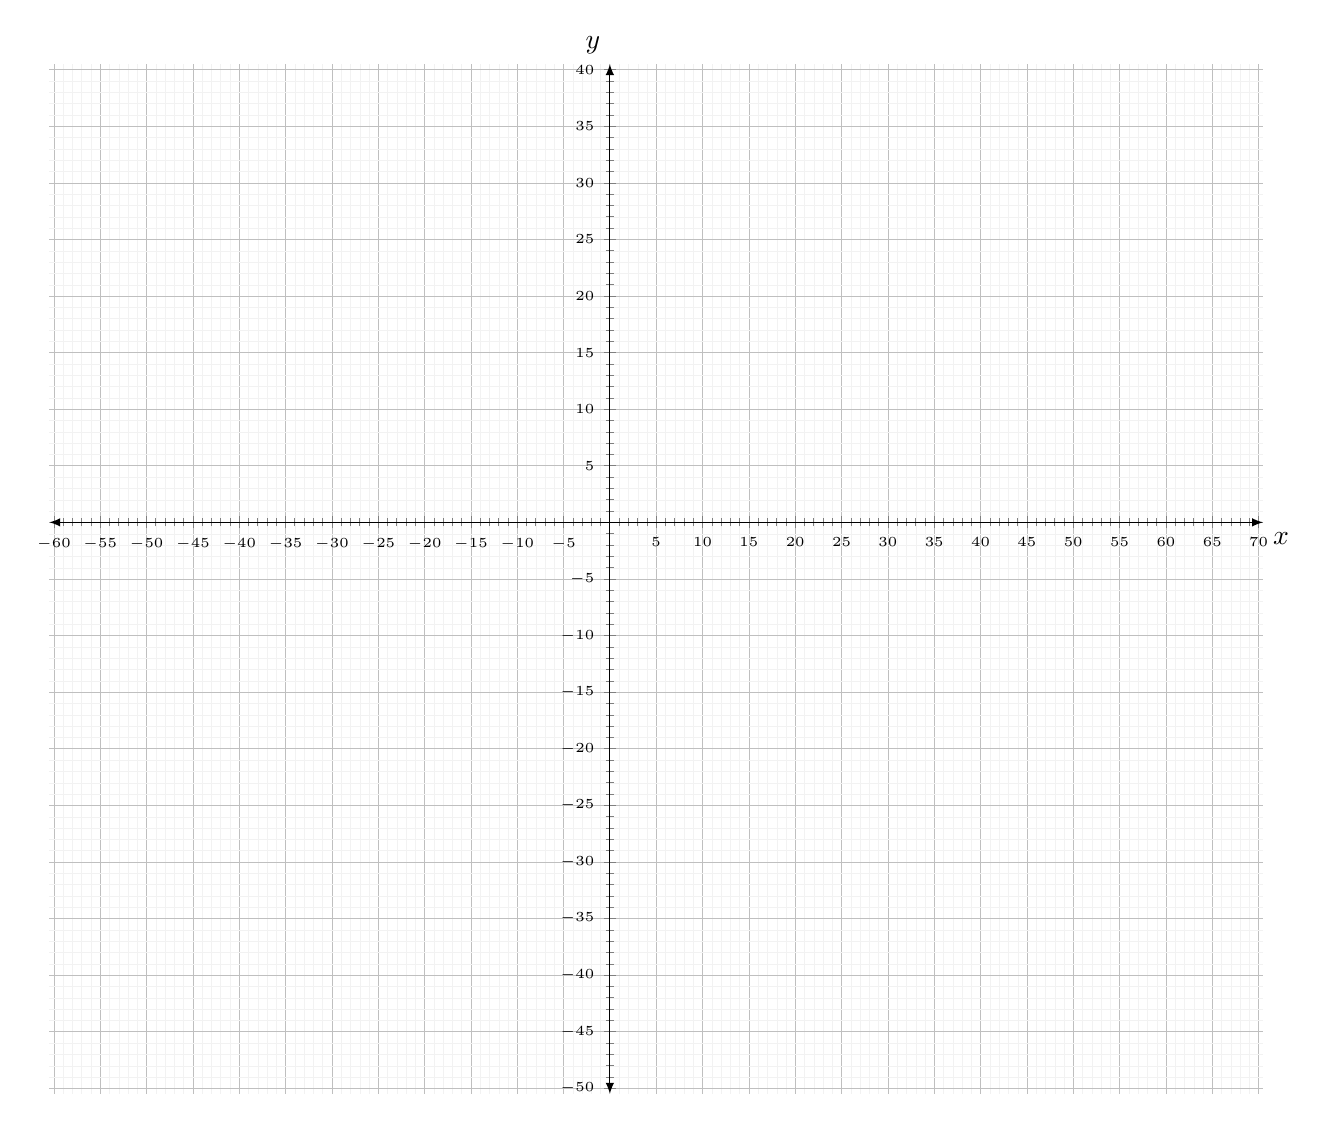
\begin{tikzpicture}[scale=1]
        \begin{axis}[
            axis x line=center,
            axis y line=center,
            xlabel = {$x$},
            ylabel = {$y$},
            xmin=-60,xmax=70,
            ymin=-50,ymax=40,
            xtick distance=5, 
            ytick distance=5, 
            grid=both,
            grid style={line width=.1pt, draw=gray!10},
            major grid style={line width=.2pt,draw=gray!50},
            axis lines=middle,
            axis line style={<->},
            minor tick num=4,
            enlargelimits={abs=0.5},
            axis line style={latex-latex},
            ticklabel style={font=\tiny},
            % ticklabel style={font=\tiny,fill=white},
            % xlabel style={at={(ticklabel* cs:1)$},anchor=north west},
            % ylabel style={at={(ticklabel* cs:1)$},anchor=south west},
            xlabel style={below right},
            ylabel style={above left},
            width=17cm,
        ]
        
        \end{axis}

    \end{tikzpicture}

\end{questions}
 
\end{document}